\documentclass{sig-alternate}

\usepackage{url}
%\usepackage[caption=false]{subfig}
\usepackage{subcaption}

%\usepackage{amssymb}
%\usepackage{amsmath}
\usepackage{color}
\usepackage{algorithm}
\usepackage{algpseudocode}
\usepackage{booktabs}
\usepackage{array}
\usepackage{xspace}
\usepackage{graphicx}

% shortcut
\newcommand{\etc}{{etc.}\@\xspace}
\newcommand{\ie}{{i.e.}\@\xspace}
\newcommand{\etal}{{et al.}\@\xspace}
\newcommand{\eg}{{e.g.}\@\xspace}
\newcommand{\aka}{{aka}\@\xspace}
\newcommand{\comment}[1] {\textbf{\color{red}{Comment: #1}}}
\renewcommand{\algorithmicforall}{\textbf{for each}}

\newtheorem{theorem}{Theorem}
\newtheorem{definition}{Definition}

\newcolumntype{L}[1]{>{\raggedright\let\newline\\\arraybackslash\hspace{0pt}}m{#1}}
\newcolumntype{C}[1]{>{\centering\let\newline\\\arraybackslash\hspace{0pt}}m{#1}}
\newcolumntype{R}[1]{>{\raggedleft\let\newline\\\arraybackslash\hspace{0pt}}m{#1}}


% \usepackage{setspace} % squeeze the vertical space in algorithm

% \makeatletter
% \renewcommand{\ALG@beginalgorithmic}{\small}
% \makeatother

\graphicspath{{figs/}}

\begin{document}

\title{A Server-side View of TCP Performance of Mobile Voice Search}
\author{}

\maketitle

%!TEX root = main.tex

\section{Introduction}
\label{sec:intro}

Voice search service has become popular over the last few years due to its convenience on mobile devices. A recent report showed that more than half of teens use voice search more than once a day~\cite{voice_search_report}. A voice search session consists of two successive phases: voice recognition and web search. First, the mobile terminal transmits the speech data to a voice recognition server and gets the recognized keyword(s). After that, the mobile terminal queries the keyword(s) and obtains the search results. The two phases are carried out across two independent flows, established to different servers. One of the flows is uploading data (voice search), the other is downloading data (web search result), and both flows are short (less than 100 packets).

In this paper, we are motivated by the fact that the latency and packet loss rates in mobile and wireless network are able to significantly degrade user-perceived performance in such voice search service. There is already a large body of work \cite{sommers2012cell,yu2014can,chen2012network,sharma2010goodput} studying the impact of network quality on user perceived performance of mobile applications. However, most of them focus on the downloading efficiency of relatively long flows in wireless and mobile network, which is not applicable to the voice search service, which contains mostly short flows, both in the upload and download directions. The complexity and uniqueness of voice search is a great opportunity to better understand the user-perceived performance in this type of traffic.

To this end, we obtained a unique dataset from voice search servers in one of the top 3 search service providers in China. The dataset spans over two weeks in April 2015, consisting of about 1 million voice recognition flows and 3 million web search flows from 3G and WiFi network, in the usual pcap format. We break down the analysis into two independent segments: voice recognition (Section~\ref{sec:voice}) and web search (Section~\ref{sec:web_search}), with emphasis on the disparity that might exist when accessing using 3G and WiFi connection. In each part, we analyze the network-related finish time of flows, and in particular the impact of TCP performance factors (i.e. RTT, packet loss/disordering, timeout retransmission) on the finish time. However, as we observe flows from the server-side, we do not have visibility of when the clients sent their TCP segments. Therefore, we propose heuristics to estimate the TCP performance factors. On the other hand, we can collect the information of all the TCP performance factors for web search flows, and thus partition a web search flow into three TCP stages: 3-way handshake, slow start, and congestion avoidance. We then examine the impact of the three stages on the finish time, and inspect the key performance parameters in each stage. Our main observations are the following:

%We focus on the disparity that might exist between TCP upload and download flows and also the possible difference when searching using 3G and WiFi connection. In particular, we analyzed timeout retransmission, an expensive operation for packet loss recovery as it dominates the finish time once it happens. We have made several key observations , which constitute valuable insights for improving the user-perceived performance in voice search service.


\begin{itemize}
\item Flows in both voice recognition and web search are short (no more than 4 packets and 100 packets respectively). Despite the small flow size, there are outlier flows experiencing extremely long finish time. For instance, we observe that 10\% of WiFi flows in voice recognition spend more than 0.5 second for voice data uploading, and 20\% of WiFi flows in web search cannot finish the search result transmission within 1 second.

\item The finish time in both voice recognition and web search is proportional to RTT when there is no packet loss. RTT however exhibits a large variation, especially in WiFi network. We observe the RTT of WiFi flows ranges from 10 ms to 400 ms with a median around 40 ms. 

\item For those flows with packet loss, the finish time is dominated by the the time for loss recovery operations, especially by timeout retransmissions. We observe that WiFi flows are more likely to suffer from timeout retransmission than 3G flows due to the higher packet loss rate (3\% in WiFi vs 0.9\% in 3G). The timeout retransmissions can even happen during connection establishment, leading to an extremely large finish time.

\item We classify timeout retransmission in web search flows into four types based on how they are triggered. Tail retransmission is the most common type in both WiFi flows (38.3\%) and 3G flows (69.6\%). However, double retransmission and packet delay retransmission are more likely to happen in WiFi flows (33.8\% and 27.4\% in WiFi versus 13.5\% and 16.1\% in 3G).

\end{itemize}

Our findings highlight the impact of TCP performance factors on the flow finish time in this peculiar but increasingly popular service. We believe that these findings provide valuable insights into the design of voice search service, the optimizations of TCP protocol for short flows of both upload and download, middlebox diagnosis, and their interactions.

The remaining of this paper is organized as follows. Section~\ref{sec:dataset} describes the dataset. Section~\ref{sec:voice} and Section~\ref{sec:web_search} carry out an in-depth analysis on the performance of voice recognition and web search separately, and inspect the performance causes. Section~\ref{sec:discuss} discusses the implication of the observations and the possible shortcomings of this work. Section~\ref{sec:related} compares the related work and Section~\ref{sec:conclude} concludes our work. 

%!TEX root = main.tex

\section{Data}
\label{sec:dataset}

We begin this section with the description of our packet-level data from a mobile voice search service, and then provide high-level statistics of TCP performance. 

\subsection{Data Collection}

\begin{figure}[th]
	\centering
	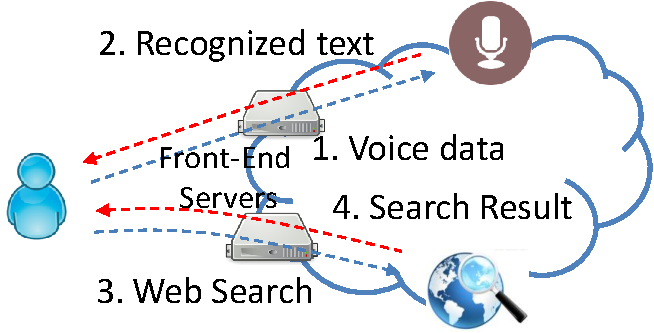
\includegraphics[width=0.8\linewidth]{voice_search_process}
	\caption{Voice search engine infrastructure.}
	\label{fig:voice_search}
\end{figure}

We collect mobile voice search data from one of the top 3 search service providers in China. This service provider serves more than 400 million users per day. A voice search initialized from a mobile terminal consists of two successive phases as shown in Figure~\ref{fig:voice_search}: \emph{voice recognition} (\ie recognize speech to query text) and \emph{web search} (\ie search with returned query text). Voice recognition and web search are served by different servers through HTTP. As such, a voice search session consists of two separate TCP flows.

We collect packet-level traces from front-end servers\footnote{Note that our traces are from a subset (3) of all servers, and given the load-balancing done across these, our data likely represents a uniform random flow sample.} of both voice recognition and web search, resulting in two datasets that correspond to the two phases of voice search. The front-end servers from which we obtained the data provide services for mobile users in the same geographical locations. As the service provider relies on geographically-biased server selection, we assume that the flows in the two datasets cross networks with similar characteristics. The web search servers provide search services for both voice search and traditional user-type search. The datasets were collected in April 2015 for two weeks. In total, we obtained about 1 million voice recognition flows and 3 million web search flows.

%We report measurement results for each of the two phases of voice search.

All voice search requests are originated from mobile apps, especially from the Android platform, either via cellular or WiFi access network. About 2.5\% of the voice recognition flows and 6.7\% of the web search flows originate from the cellular network, made of a mixture of technologies: 2.5G, 3G and 4G\footnote{The cellular network type was inferred using the HTTP header field ``x-up-bear-type''.}. However, we observed a very limited number of 2.5G and 4G flows (less than 0.5\% of the total flows) in our data\footnote{Indeed, 4G is still in its initial stages of deployment in China and has limited coverage.} and thus omit them from our analysis. In total, they make up about 2.5\% of the flows.

\begin{figure}[th]
\centering
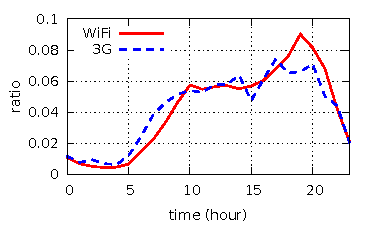
\includegraphics[width=0.8\linewidth]{voice_time_rate}
\caption{Distribution of voice search requests in a day.}
\label{fig:voice_time_rate}
\end{figure}

Figure~\ref{fig:voice_time_rate} shows the distribution of voice search flows over time of a day. Flows are binned into 1-hour frame and we report the ratio of flows in each interval divided by the daily total. Not surprisingly, we observe a sharp increase of the search volume from 5AM to 10AM. The search volume from 3G remains relatively stable over the day and declines around 10PM, while we observe continuous growth of the WiFi search which reaches its peak at 7PM. The daily trend for web search flows is similar (not show). The daily search volume variation trend we observe is very similar to the one previously reported by \cite{Song:2013:EEU:2488388.2488493} for Bing mobile search.

\subsection{TCP Performance Measures}

\begin{figure}[ht]
\centering
\begin{subfigure}[b]{0.6\linewidth}
	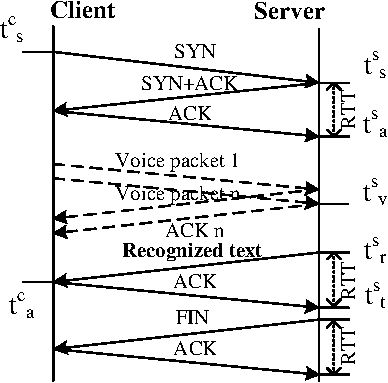
\includegraphics[width=\textwidth]{voice_estimate_rtt}
\caption{Voice recognition}
\label{fig:voice_estimate_rtt}
\end{subfigure} \\
%\vspace{0.1in}
\begin{subfigure}[b]{0.6\linewidth}
	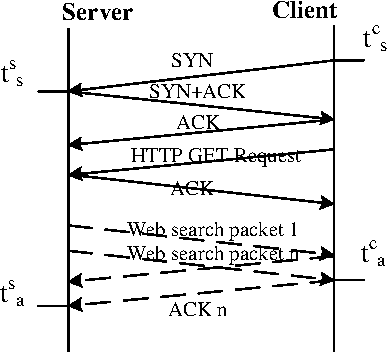
\includegraphics[width=\textwidth]{web_finish_time_example}
\caption{Web search}
\label{fig:web_finish_time_example}
\end{subfigure}
\caption{Time-line of a voice recognition flow and a web search flow.}
\label{fig:time_line}
\end{figure}

% For a voice search session, both the voice recognition and the web search phases contribute to the performance. However, they could have very distinct behavior as seen from the server-side. This is because as shown in Figure \ref{fig:time_line}, in the voice recognition phase, the server acts as a TCP receiver, while in the web search phase, the server is the sender. Note that TCP is largely a sender-driven transmission protocol and its transmission performance is affected by the ability of the sender to handle congestion events, as well as the ability of the receiver to receive data. We examine the TCP performance factors of each phase for individual voice search sessions and their impact on the flow \emph{flow completion time}.

User perceived response time of a mobile voice search session is affected by the \emph{completion time} of the voice recognition flow as well as that of the web search flow. Here, the completion time of a flow measures the duration from the time when client initiates the connection till the time when the last byte of data is acknowledged. We define the completion time for the flows in the two phases separately as follows.

Voice recognition consists of mobile terminals uploading the voice data and server returning back the recognized query text as shown in Figure~\ref{fig:voice_estimate_rtt}. The following web search is initialized by mobile clients once they receive the recognized text (encapsulated in one packet) at $t^c_a$. That said, the completion time of a recognition flow measures the duration from $t^c_s$ to $t^c_a$. Unfortunately, we do not have these two timestamps at server side where we collected our datasets. Note that the timestamp option in TCP is disabled since otherwise, clients behind NATs (Network Address Translations) might not be able to build connections with the servers that with PAWS (Protect Against Wrapped Sequence number) \cite{rfc7323} enabled \cite{Wang:2011:USM:2018436.2018479}. Alternatively, we approximate the flow completion time with $T_s=t^s_t - t^s_s$. This flow completion time however includes the time consumed by servers to translate speech to text ($T_r=t^s_r - t^s_v$), which is not relevant to network performance\footnote{The time duration needed for translating voice to text is dependent on the used speech recognition technology. We refer interested readers to \cite{36463,schalkwyk2010your} for more details regarding speech recognition.} and therefore out of scope in this paper. We thus redefine the flow completion time of a voice recognition flow as $T_s-T_r$.

Web search starts when a mobile terminal initiates a connection to transmit the query text, and ends when the server receives ACKs for all returned search results as shown in Figure~\ref{fig:web_finish_time_example}. Note that for the web search phase, we only consider flows carrying search results that are dynamically generated by servers based on the query and ignore those corresponding to static content such as CSS/JavaScript files. This is because the performance for static content (as opposed to the dynamic search results) can be optimized easily through CDN (Content Delivery Network) caching. The flow completion time at the client-side is the duration between transmitting the SYN packet $t^c_s$ and receiving all web search data $t^c_a$. We use the duration $T_s=t^s_a - t^s_s$ measured at the server-side to approximate the latency that the user perceives. Again, we excluded the time consumed by servers processing the query $T_r=t^s_r - t^s_q$ and obtained the flow completion time as $T_s-T_r$.

\begin{figure}[t]
\centering
\begin{subfigure}[b]{0.8\linewidth}
	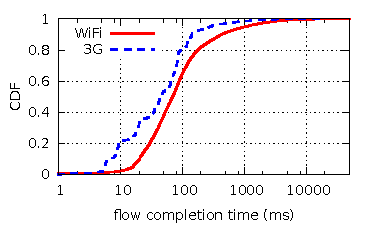
\includegraphics[width=\textwidth]{voice_finish_time}
\caption{Voice recognition}
\label{fig:voice_finish_time}
\end{subfigure} \\
%\vspace{0.1in}
\begin{subfigure}[b]{0.8\linewidth}
	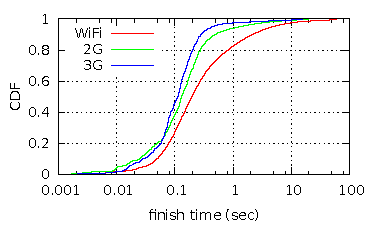
\includegraphics[width=\textwidth]{web_finish_time}
\caption{Web search}
\label{fig:web_finish_time}
\end{subfigure}
\caption{CDFs of flow completion time in the two phases.}
\label{fig:finish_time}
\end{figure}


Figure~\ref{fig:finish_time} plots the cumulative distribution (CDF) of the flow completion time of TCP flows in the two phases, where $x$-axis is in log scale. Interestingly, we find that in both phases 3G flows experience a shorter completion time than WiFi flows. Furthermore, some flows experience a very large completion time compared to others, displaying a heavy tailed behavior that was also found in Google search \cite{flach2013reducing}. For example, while most of the voice recognition flows finish in 100ms, a non-negligible fraction of flows (5\% in WiFi, and 2\% in 3G) take more than 1 second to upload the voice data. 

%Figure~\ref{fig:web_finish_time} shows the CDF of flow completion time of web search flows. In the figure, the overall completion time of flows in 2G and 3G (with median values 0.013s and 0.011s) in also shorter than that of flows in WiFi network (with median value 0.2s). More than 25\% of flows in all networks experience completion time less than 0.1 second. However, 5\% of flows in 2G network and 18\% in WiFi network experience completion time more than 1 second. Furthermore, about 3\% of flows in WiFi network are with completion time more than 10 seconds, which is a great performance degradation.

A comparison of the TCP flow completion time between voice recognition and web search in Figure~\ref{fig:finish_time} shows that the flow completion time in web search contributes to the majority of the user-perceived (network-related) performance of a voice search session. However, it does not mean that understanding the performance of voice recognition flows is not as important as for web search flows. Indeed, voice recognition is the first step of the whole voice search process, and therefore a long recognition time would certainly result in bad user experience, potentially even early termination of the process.

% These observations motivate our analysis of the TCP performance and its impact on the flow completion time in each phase of the mobile voice search.

% some of voice recognition flows suffer from timeout retransmission, which is a great performance degradation~\cite{flach2013reducing}. Second, a non-negligible fraction of voice recognition flows are terminated before voice data transmission completes. These bad user experiences also inspire us to understand what factors and how they impact user-perceived performance in voice recognition flows.

We were motivated by the above observations to have an in-depth analysis of the TCP performance in mobile voice search. To this end, we focus on the following three most important aspects of TCP performance.

\begin{itemize}
	\item {Round Trip Time (RTT):} RTT is a commonly used indicator of TCP performance, especially for short TCP flows like search flows.
	
	\item {Number of lost/disordered packets:} Both packet loss and packet reordering could affect the transmission time. Packet loss leads to a reduction of the sender congestion window. Although packet reordering does not reduce the congestion window, it can prevent the congestion window from growing and may trigger spurious retransmissions.
	
	\item {Timeout Retransmission:} In timeout retransmission, the TCP sender has to wait for a RTO (Retransmission Timeout) before retransmitting the lost packet. The RTO can be tens of RTTs. Such kind of ``expensive'' retransmissions can degrade TCP performance, especially for short flows like those considered in this paper~\cite{flach2013reducing}.

\end{itemize}

%When examining the impact of the above factors on TCP flow completion time, we also consider the potential impact of TCP flow size. We are particularly interested in the disparity that might exist when issuing voice searches from 3G and WiFi. 
TCP is a sender-driven transmission protocol and its performance is mainly affected by the sender-side factors. However, as shown in Figure \ref{fig:time_line}, the server acts as a TCP receiver in the voice recognition phase. As such, we cannot obtain the statistics of the above TCP performance factors of the sender in the voice recognition phase. Alternatively, we infer as much information as we can for these factors. The server in the web search phase is on the other hand the TCP sender, and thus we can have a better view of how the TCP sender behavior and its impact on the flow completion time. In addition, we are particular interested in the disparity that might exist when issuing voice searches from 3G and WiFi. 

%!TEX root = main.tex

\section{Understanding Voice Recognition Performance}
\label{sec:voice}

\begin{table*}[t]
\caption{High-level statistics of voice recognition flows.}
\label{tab:voice_stats}
\centering
\renewcommand{\arraystretch}{1.0}
\begin{tabular}{c|C{2.6cm}|c|c|C{2.1cm}|C{2.1cm}}
	\hline
	& Flow completion time (ms) & Flow size (\#pkts) & RTT (ms) & \% of flows w/ reord. pkts & \% of flows w/ timeout retx \\
	\hline
	WiFi & 69 (15, 1,052) & 3.0 (2.0, 4.0) & 45 (12, 399) & 3.3\% & 6.7\% \\
	%\hline
	3G & 55 (6, 316) & 3.0 (2.0, 4.0) & 35 (5, 99) & 6.6\% & 6.1\% \\
	\hline
\end{tabular}
\minsqueeze
\end{table*}

%\begin{figure}[th]
%	\centering
%	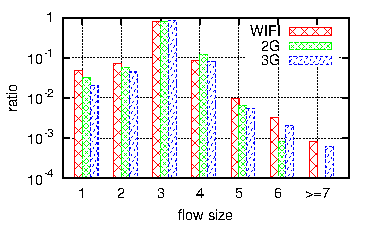
\includegraphics[width=0.8\linewidth]{voice_flow_size}
%	\caption{The number of voice data packets in voice recognition flows.}
%	\label{fig:voice_flow_size}
%\end{figure}

In this section, we look at TCP performance of voice recognition flows. We first provide high-level statistics on key performance indicators for 3G and WiFi flows in Table~\ref{tab:voice_stats}. For flow completion time, flow size and RTT, we report the median along with the $5th$ and $95th$ percentiles in parenthesis. The flow size is measured in number of data packets. Independent of the access technology, nearly all voice recognition flows contains no more 4 data packets. Given that the initial congestion window in the current Android TCP/IP stack is set to 10 segments~\cite{dukkipati2010argument}, the data can be transmitted in the initial congestion window. Another interesting observation from Table~\ref{tab:voice_stats} is that 3G flows tend to have smaller RTTs but a higher probability of suffering from packet reordering. In what follows, we examine each TCP performance factor and its impact on the flow completion time.

\subsection{RTT}

As illustrated in Figure~\ref{fig:voice_estimate_rtt}, we can measure at most 3 RTTs at the server-side in a voice recognition flow. However, the RTT is ambiguous when segments are retransmitted. To address this, we use the following methodology to determine the \emph{minimal RTT}. If no retransmission happens for SYN packets, $t^s_a - t^s_s$ is used as the RTT of the flow, \ie the RTT is measured during the 3WHS (3-way handshake). Otherwise, the RTT measured during connection termination is preferred if the FIN packet is not retransmitted. In the case that both of the above RTTs are ambiguous, $t^s_t - t^s_r$ is used as the measured RTT. We have verified using our datasets that the RTT measured during 3WHS is the minimal RTT in more than 60\% of flows, and is less than 2 times of the minimal RTT in 95\% of flows. We believe that it is reasonable to assume that the RTT measured using the above methodology is close to the minimal RTT of the flow at client-side, and the most representative of the network latency.

Figure~\ref{fig:voice_rtt} plots the distribution of RTTs measured in individual voice recognition flows. The median RTT of 3G flows is around 35 ms. WiFi flows on the other hand exhibit a larger RTT with a median around 45 ms. In particular, while 95\% of 3G flows have a RTT less than 100 ms, about 20\% of WiFi flows have a RTT larger than this value.

\begin{figure}[t]
\centering
	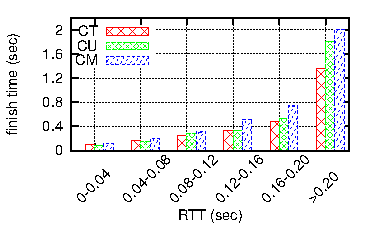
\includegraphics[width=0.8\linewidth]{voice_rtt}
\caption{RTTs in voice recognition flows.}
\label{fig:voice_rtt}
\minsqueeze
\end{figure}

\begin{figure}[th]
\centering
	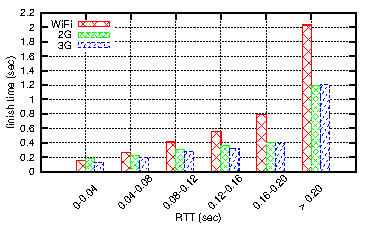
\includegraphics[width=0.8\linewidth]{voice_rtt_finish_time}
\caption{Impact of RTT on flow completion time for voice recognition flows.}
\label{fig:v_rtt_time}
\minsqueeze
\end{figure}

We further examine the impact of RTT on flow completion time in Figure~\ref{fig:v_rtt_time}. We observe that for flows having a RTT no larger than 200 ms, the flow completion time increases with the RTT: the ratio of flow completion time to RTT is about 2.5 for 3G flows and about 4 for WiFi flows. Since the completion time of a voice recognition flow is approximately 2 RTTs (in which 1 RTT for building connection, and 1 RTT for uploading data), the difference of the ratio between cellular network and WiFi network should come from the data uploading time. One possibility is that the RTT during data transfer in WiFi is significantly higher than the RTT measured during connection establishment (\ie 3WHS) \cite{UM-CS-2012-022}, where we obtained most of the RTTs. It seems that 3G networks provide consistent RTTs during the flow lifetime.

The flow completion time becomes extremely large when the RTT is larger than 200ms. Such an RTT could be an indication of network congestion, as the servers are likely to be geographically close to the clients. In other words, it is likely that the flow is traversing a congested network and may encounter packet loss, which takes a relatively long time for recovery.

\subsection{Packet Reordering}
\label{sec:v_pd}

\begin{figure*}[th]
\centering
	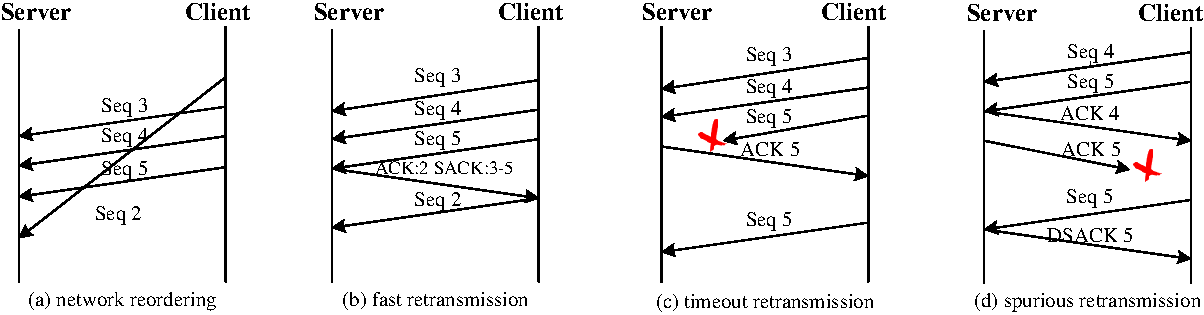
\includegraphics[scale=0.7]{voice_flow_estimate_retrans}
\caption{Server could not distinguish packet reordering events, which are (a) packet reordering, (b) fast retransmit, and (c) timeout retransmission. Server may identify some timeout retransmissions as long packet delay (d).}
\label{fig:voice_flow_estimate_retrans}
\minsqueeze
\end{figure*}

Another factor that can heavily impact the flow completion time are network congestion events, which can be observed by servers as packet loss, packet delay and packet reordering. However, as a TCP receiver, the server might not be able to infer the type of network congestion event. For example, the server observes the same packet sequences for Figure~\ref{fig:voice_flow_estimate_retrans}(a), \ref{fig:voice_flow_estimate_retrans}(b) and \ref{fig:voice_flow_estimate_retrans}(c), despite that they depict 3 types of congestion: packet reordering in Figure~\ref{fig:voice_flow_estimate_retrans}(a), fast retransmit for packet loss recovery in Figure~\ref{fig:voice_flow_estimate_retrans}(b) and timeout retransmission for packet loss recovery in Figure~\ref{fig:voice_flow_estimate_retrans}(c). These observations illustrate the challenge in TCP analysis of uploading flows from the server-side.

We use the number of reordered packets, a metric that the server can compute, to capture the network congestion characteristics. In the examples shown in the first 3 subfigures in Figure~\ref{fig:voice_flow_estimate_retrans}, the number of reordered packets is 1. %As we have shown in Figure~\ref{fig:voice_flow_estimate_retrans}, a reordered packet seen by the serve could be caused by either packet reordering, fast retransmit or timeout retransmission for packet loss recovery (i.e. Figure~\ref{fig:voice_flow_estimate_retrans}(a-c)). 
We report the percentage of flows with packet reordering in Table~\ref{tab:voice_reorder}.

\begin{table}[th]
\caption{Percentage of flows with packet reordering.}
\label{tab:voice_reorder}
\centering
\renewcommand{\arraystretch}{1.0}
\begin{tabular}{c|c|c|c}
	\hline
	\# reord. pkts & 0 & 1 & $\ge$2 \\
	\hline
	WiFi & 96.7\% & 3.03\% & 0.2\% \\
	\hline
	3G & 93.3\% & 6.6\% & - \\
	\hline
\end{tabular}
\minsqueeze
\end{table}

As expected, the majority of flows experience no packet reordering. However, we observe that 6.6\% of 3G flows and 3\% of WiFi flows have one reordered packet. The fraction of flows having more than 2 reordered packets is negligible. Given that in most cases, the voice data only consists of 3 packets, just a single reordered packet can severely impair flow performance as shown in Figure~\ref{fig:voice_reorder}.

\begin{figure}[th]
\centering
	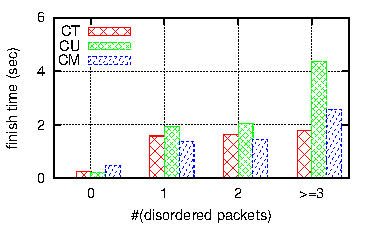
\includegraphics[width=0.8\linewidth]{voice_reorder}
\caption{Impact of packet reordering on flow completion time.}
\label{fig:voice_reorder}
\minsqueeze
\end{figure}

We can see from Figure~\ref{fig:voice_reorder} that one reordered packet in 3G uploading flows can increase the median flow completion time from 10 ms to 60 ms. For WiFi flows, we observe as many as 20\% of the flows suffering from packet reordering cannot finish the upload within 1 second. When receiving a reordered packet, the server feeds back to the client with a SACK (as shown in Figure~\ref{fig:voice_flow_estimate_retrans}). The client will retransmit the packet in the hole (\ie the reordered packet) after collecting 3 SACKs. In the case that too few SACKs can be collected, the client has to rely on the expensive timeout retransmission mechanism for recovery. %That said, the increased flow completion time might be caused by either packet delay, fast retransmit or timeout retransmission. Unfortunately, we cannot identify how much each of these congestion events contributes using the datasets collected from server side.

The significance of the impact of packet reordering on flow completion time is also dependent on RTT, as both the waiting time for fast retransmit and timeout retransmission timer (\ie RTO) depend on the RTT. To further assess the impact of packet reordering by excluding the possible effect of other covariates (\eg RTT), we rely on non-parametric factorial analysis using a Quasi Experimental Design (QED) \cite{krishnan2013video}. In QED, each uniformly sampled individual $u$ is compared with an individual $v$ randomly selected from those that have identical covariates with $u$ except the cause variable (packet reordering in our context). Any difference in outcome between these two individuals can be attributed to the cause variable we are tracking.

We bin for each access technology the voice recognition flows into two groups: those with no reordered packet ($G_1$) and those with 1 reordered packet ($G_2$). For each flow $u \in G_1$, we randomly choose a flow $v$ from $G_2$ that has similar RTT (\ie the difference is less than 40 ms) and the same condition in terms of timeout retransmission as identified by the methodology from Section~\ref{sec:v_rto}. We record the outcome difference as $o_{u,v} = \frac{ftime_{v} - ftime_{u}}{ftime_{u}}$, where $ftime_v$ is the completion time of the flow $v$. Finally, we average all outcome differences over the matched pairs and use this average difference to gauge the impact of packet reordering.

\begin{table}[th]
\caption{QED results for the impact of packet reordering.}
\label{tab:voice_qed_reorder}
\centering
\renewcommand{\arraystretch}{1}
\begin{tabular}{C{1cm}|C{1.5cm}|C{1.5cm}}
	\hline
	 & WiFi & 3G \\
	\hline
	QED & 6.42 & 4.45 \\
	\hline
\end{tabular}
\minsqueeze
\end{table}

Table~\ref{tab:voice_qed_reorder} presents the QED results, which show that one reordered packet can lead to an increase of flow completion time by a factor as large as $4-6$. The larger flow completion time increase of WiFi compared to 3G flows is due to the packet reordering events in WiFi flows that are more likely to originate in packet losses (\ie Figure \ref{fig:voice_flow_estimate_retrans}(b) and \ref{fig:voice_flow_estimate_retrans}(c)), which require more time to recover. Indeed, we find using the web search dataset that the packet loss rate in WiFi is 3.0\% compared to 0.9\% in 3G\footnote{We cannot obtain the packet loss rate of voice recognition flows as the server where we collected our dataset is a TCP receiver.}. 

\subsection{Timeout Retransmissions}\label{sec:v_rto}

\begin{figure}[th]
\centering
	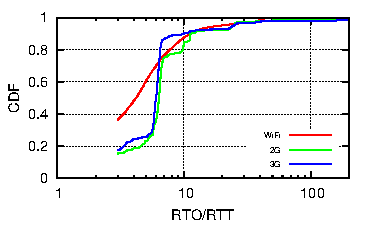
\includegraphics[width=0.8\linewidth]{voice_rtt_rto_ratio}
\caption{Distribution of RTO/RTT.}
\label{fig:rto_rtt}
\minsqueeze
\end{figure}

We rely on the time gap between actual arrival time and the estimated arrival time of individual packets to infer timeout retransmissions in voice recognition flows. We observe a behavior similar to Figure~\ref{fig:voice_flow_estimate_retrans}(d). The estimated arrival time of a packet is the mean value of the arrival time of the previous packet and subsequent packets. If this gap is larger than a RTO, the transmission of the packet is identified as a timeout retransmission. However, the server does not know the client-side RTO, which has to be estimated. The RTO in the TCP implementation is set to $\text{SRTT} + max(200ms, 4 \text{ RTTVAR})$\cite{rfc62982011computing}, where SRTT is close to RTT, and RTTVAR is approximately $RTT/2$, \ie $$\widehat{RTO} \approx RTT + max(200ms, 2 RTT) \enspace .$$ Note that the timeout retransmissions identified using the above methodology do not overlap with those shown in Figure~\ref{fig:voice_flow_estimate_retrans}(c).

We first examine how large RTOs can be in Figure~\ref{fig:rto_rtt}, where we plot the distribution of RTO/RTT. We can observe the median RTO is around 4-6 times the RTT, but can be as large as tens of RTTs. Given that a time retransmission takes a RTO for recovery, the impact of timeout retransmission on flow completion time can be significant.

\begin{table}[th]
\centering
\renewcommand{\arraystretch}{1.1}
\caption{Flows with timeout retransmission.}
\label{tab:voice_timeout_stats}
\begin{tabular}{c | C{2cm} | C{2cm}}
	\hline
	 & WiFi & 3G \\
	\hline
	3WHS retx & 2.6\% & 0.8\% \\
	%
	data retx & 6.7\% & 6.1\% \\
	\hline
\end{tabular}
\minsqueeze
\end{table}

Table~\ref{tab:voice_timeout_stats} lists the percentage of flows that suffer from at least one timeout retransmission in our dataset. The timeout retransmission could happen either during the 3WHS or data transmission. While the timeout retransmission during 3WHS is less likely to happen compared to timeout retransmission during data upload, its impact might be even larger. This is because the initial RTO is set to 1 second~\cite{rfc62982011computing} as there is no RTT available at that time. This RTO value is often much larger than the one computed during data upload. Users might quit the app during this the period taken for recovery. In addition, a timeout retransmission during the 3WHS results in the congestion window size going to 1, which further impairs the performance for data transmission.

Regardless of the access technology, we observe as many as over 6\% of the voice data upload flows suffering from at least one timeout retransmission. Such a large fraction of timeout retransmission flows can be explained by the fact that almost all the voice recognition flows contain no more than 4 voice data packets. When one of the last three packets is dropped, the sender (\ie client) has to wait RTO for retransmission. This behavior is similar to the tail loss identified in~\cite{flach2013reducing}. In the voice data upload context, the server is no longer a sender and thus unable to eliminate such kind of RTO retransmissions by gently sending redundant packets as proposed in~\cite{flach2013reducing}. Our results highlight the need for TCP optimizations for uploading flows at the server-side. 

\begin{figure}[th]
\centering
	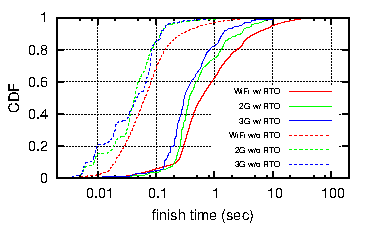
\includegraphics[width=0.8\linewidth]{voice_timeout}
\caption{CDF of flow completion time with and without timeout retransmission.}
\label{fig:voice_rto}
\minsqueeze
\end{figure}

\begin{table*}[t]
\caption{High-level statistics of web search flows.}
\label{tab:web_stats}
\centering
\renewcommand{\arraystretch}{1.0}
\begin{tabular}{c|C{2.6cm}|c|c|C{1.2cm}|C{1.85cm}|C{2.1cm}}
	\hline
	& {Flow completion time (ms)} & {flow size (\#pkts)} & {RTT (ms)} & pkt loss rate & \% of flows w/ lost pkts & \% of flows w/ timeout retx \\
	\hline
	WiFi & 197 (30, 4,608) & 9.0 (1.0, 33.0) & 39 (10, 372) & 3.0\% & 9.76\% & 4.1\% \\
	\hline
	3G & 124 (15, 440) & 19.0 (1.0, 82.0) & 38 (4, 68) & 0.9\% & 8.7\% & 0.1\% \\
	\hline
\end{tabular}
\minsqueeze
\end{table*}

We finally compare the completion time between flows with and without timeout retransmission in Figure~\ref{fig:voice_rto} (note the log scale $x$-axis). The timeout retransmission increases the median flow completion time from 64ms to 595ms, \ie one order of magnitude larger. This is not surprising given that RTO is several times larger than the RTT. Perhaps more importantly, we observe that 10\% of WiFi flows with timeout retransmissions require as much as 5 seconds to upload the voice data. The voice search sessions that correspond to these flows are indeed likely to be terminated by users. In fact, since the number of voice data packets is relatively small ($\le 4$), which can be uploaded within 2 RTTs, the retransmission time (\ie RTO) will dominate the flow completion time of the flows experiencing timeout retransmissions.  Overall, a larger fraction of WiFi flows suffer from timeout retransmission compared to 3G flows, which partially explains their larger flow completion time observed in Figure~\ref{fig:voice_finish_time}.

\subsection{Summary of Voice Recognition Analysis}

The key observations on voice recognition flows are summarized as follows:
\begin{itemize}
\item Most of voice recognition flows contain no more than 4 data packets, which fit into the initial congestion window of the client. Ideally, the voice data can be transmitted in 1 RTT.
\item For flows with smaller RTT (say no more than 200 ms), the flow completion time is proportional to RTT. WiFi flows tend to have larger flow completion time compared to those in 3G, due to larger RTT. 	
\item Reordered packets, caused by either packet delay or packet loss, increasing the flow completion time by 4-6 times. Although WiFi flows are less likely to see reordered packets than 3G flows, they suffer more from packet reordering due to longer time for recovery.
\item Timeout retransmission, which can happen either during connection establishment or during data transfer, increases the flow completion time by as much as one order of magnitude. In addition, WiFi flows suffer more from timeout retransmissions than 3G flows.
\end{itemize}
%!TEX root = main.tex

\section{Understanding Web Search Performance}
\label{sec:web_search}

\begin{table*}[th]
\caption{Statistics of web search flows.}
\label{tab:web_stats}
\centering
\renewcommand{\arraystretch}{1.0}
\begin{tabular}{c|c|c|c|C{1.2cm}|C{1.85cm}|C{2.1cm}}
	\hline
	& {finish time (sec)} & {flow size (\#pkts)} & {RTT (sec)} & pkt loss rate & \% of flows w/ lost pkts & \% of flows w/ timeout retrx \\
	\hline
	WiFi & 0.197 (0.030 4.608) & 9.0 (1.0 33.0) & 0.039 (0.010 0.372) & 3.0\% & 9.76\% & 4.1\% \\
	\hline
	3G & 0.124 (0.015 0.440) & 19.0 (1.0 82.0) & 0.038 (0.004 0.068) & 0.9\% & 8.7\% & 0.1\% \\
	\hline
\end{tabular}
\end{table*}

Web search starts when mobile terminal initiates connection to transmit query text, and ends when server receives ACKs for all returned search results. Figure~\ref{fig:web_finish_time_example} shows the typical time-line in web search flows. The finish time at client side is the duration from transmitting SYN packet $t^c_s$ to receiving all web search data $t^c_a$. We use the duration $T_s=t^s_a - t^s_s$ measured at server side to approximate the latency that user perceives. Again, we excluded the time consumed by servers processing the query $T_r=t^s_r - t^s_q$ and obtained the finish time as $T_s-T_r$.

For each data packet which is not retransmitted, the measured RTT is the duration from that server transmits the packet, to that server receives the acknowledgment for it. In web search progress, we record as many RTT's as possible. When each new RTT is measured, the RTO value is updated by $RTO = SRTT + max(200ms, 4 RTTVAR)$, where $SRTT$ and $RTTVAR$ mean smoothed RTT and RTT variation respectively. For a retransmitted packet, if the duration between its retransmission time and the time that last packet is transmitted is larger than the calculated RTO, we could infer that it is a timeout retransmission. For each retransmitted packet, if server would not receive D-SACK, such a retransmission recovers a real packet loss, otherwise, the packet is not dropped and the retransmission is spurious. Note that a data segment could be retransmitted twice or more if the previously retransmitted packet is regarded as lost.

In the above, we have seen that finish time in voice recognition is strongly related to the RTT value. Here we investigate the impact of RTT on finish time of web search flows. The distribution of RTT in web search is similar to that in voice recognition, which is not shown due to space limit. We use Kendall correlation to determine their relationship. The coefficient between RTT and finish time is 0.15, showing weak relationship between them. The reason is as follows. Web search result usually contains more than 10 data packets (shown in Figure~\ref{fig:web_flow_size}), which could be transmitted in 1 RTT. Moreover, how many data packets could be transmitted in one RTT is determined by congestion window size, which varies when receiving acknowledgment and packet loss event. Flows have different congestion window sizes due to different amount of congestion events in the paths they traverse. Thus RTT has limited impact on finish time in web search. 

\begin{figure}[th]
\centering
	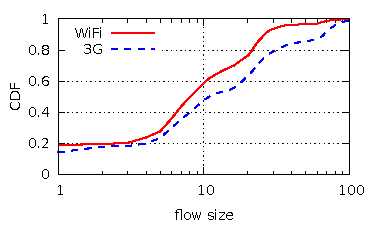
\includegraphics[width=0.8\linewidth]{web_flow_size}
\caption{The distribution of flow sizes in web search.}
\label{fig:web_flow_size}
\end{figure}

Figure~\ref{fig:web_flow_size} plots the distribution of flow size (measured by the number of web search result packets) in web search. The flow size varies from 1 packet to 100 packets with a median around 10 packets. Such a small flow size implies that any TCP performance degradation (like a high packet loss) could exert a large impact on the user perceived latency (i.e. finish time) \cite{flach2013reducing}. We also observe a smaller flow size of WiFi search than that of 3G search, which might be due to the difference in search behavior \cite{Song:2013:EEU:2488388.2488493}. We use Kendall correlation to determine whether flow size is relevant to finish time. The coefficient is 0.018, which demonstrates their irrelevance.

As a TCP sender in web search, the server can measure abundant TCP performance factors and behavior, enabling us to perform a detailed analysis of the TCP performance and its impact on the finish time. In what follows, we first characterize the finish time distribution in 3 TCP stages and then examine the impact of TCP performance factors.

\subsection{TCP Stage Analysis}

\begin{figure}[th]
\centering
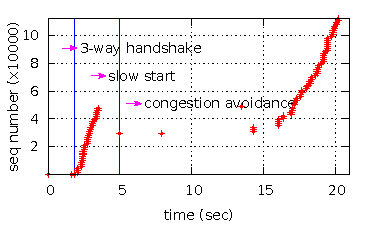
\includegraphics[width=0.8\linewidth]{web_three_stages}
\caption{The three stages in web search flows.}
\label{fig:web_three_stages}
\end{figure}

A TCP comprises 3 stages: \emph{3-way handshake}, \emph{slow start}, \emph{congestion avoidance}, which is exemplified in Figure~\ref{fig:web_three_stages} using a web search flow from our dataset, where $y$-axis shows the TCP sequence number. The TCP 3-way handshake (3WHS) stage ideally (i.e. without packet loss, delay and reordering) completes within 1 RTT. The server then enters the slow start stage, during which server does not encounter any packet loss or reordering event, and thus enlarges the congestion window by 1 segment size for each received ACK. The server enters congestion avoidance stage once it estimates a packet loss\footnote{The packet can actually be delayed or lost.}. In this stage, the server reduces the congestion window when detecting packet loss through fast retransmit\cite{rfc6675} and compels the congestion window to grow from 1 segment size when detecting packet loss through RTO. Note that the congestion avoidance stage here starts when server detects congestion event and ends till the flow finishes, which is slightly different from the TCP congestion avoidance stage in TCP/IP stack \cite{jacobson1988congestion}.

%Figure~\ref{fig:web_three_stages} gives an exemplified flow with 3 TCP stages that we define. The $y$-axis shows the TCP sequence number. In the figure, server takes 1.8s to establish connection, 3.1s to transmit 35 data packets in slow start stage, and 15.3s to transmit the left 48 data packets in congestion avoidance stage. In the following, we use the criteria of partitioning to break the analysis down into the three stages that flows experience.

\subsubsection{3-way Handshake}

\begin{figure}[th]
\centering
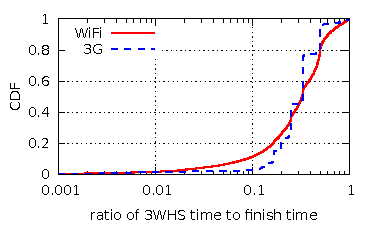
\includegraphics[width=0.8\linewidth]{web_handshake_time_ratio}
\caption{The ratio of time in 3-way handshake to finish time in each flow.}
\label{fig:web_handshake_ratio}
\end{figure}

We first examine how much of the time spent in the 3WSH stage in Figure~\ref{fig:web_handshake_ratio}, where we plot the ratio of the time in 3WSH to the finish time. Note that the $x$-axis is in log scale. 3G and WiFi flows spend similar ratio of time in this stage. We observe that the time for connection establishment can take up to half of the finish time for 30\% flows. More surprisingly, about 8\% of the WiFi flows and 3\% of 3G flows spend 70\% of their time during this stage. The small flow size is one of the reason for this observation. The maximum flow size is around 100 packets as shown in Figure \ref{fig:web_flow_size}, implying the data can be transmitted within only a few RTTs if no congestion event happens. such a short period of transmission time leads to a relatively large portion of time for connection establishment.


%From the figure, flows in cellular network have similar ratio of time in 3-way handshake to that in WiFi network (with median value 0.3). If the 3WSH could be removed from finish time, the user-perceived web search latency would be reduced by 30\% in more than half of the flows. Moreover, there are 8\% of flows in WiFi network consuming 70\% of their time in 3WSH.

%The unexpectedly high ratio of 3WSH could be introduced by two reasons. First, most of web search flows contains packets ranging from 1 to 100, these data could transmitted in 1 to 4 RTT's if there is no congestion event. Thus 3WHS, without transmitting any data, occupies a large fraction of time in short flows. Second, there are a non-negligible fraction of flows experiencing SYN retransmission during 3WHS stage. 

Another important reason that explains the unexpectedly long time in 3WSH stage (i.e. $>70\%$ of finish time) is the timeout retransmissions in this stage. As the data packets cannot be transmitted before a TCP connection is established, a loss of SYN will lead to a timeout retransmission, which takes 1 second (\ie the initial RTO) to retransmit the SYN.  We find that 4.4\% of WiFi search flows and 0.5\% of 3G flows experience at least one SYN timeout retransmission. We envision a possible way to mitigate the costly 3WSH in such short flows where clients maintain long-term TCP connections to the web search servers.

\subsubsection{Slow Start Stage}

\begin{figure}[th]
\centering
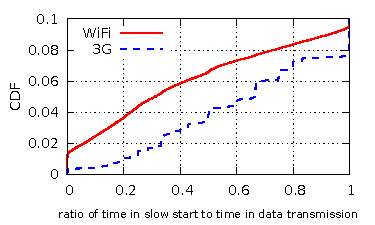
\includegraphics[width=0.8\linewidth]{web_slowstart_time_ratio}
\caption{The ratio of time in slow start to the time in data transmission.}
\label{fig:web_ss_time_ratio}
\end{figure}

The slow start stage and the congestion avoidance stage constitute the data transmission period. Intuitively, a longer time in slow start stage, the shorter time to complete the data transmission. Figure~\ref{fig:web_ss_time_ratio} shows the ratio of time in slow start stage to the time spent in data transmission (\ie the sum of time in slow start and congestion avoidance stages). Note that the $y$-axis is capped at 0.1. Regardless of the access type, more than 90\% of the flows can be finished in the slow start stage. In other words, about 10\% of the flows have to experience the congestion avoidance stage, which could lead to an increased finish time as we will see in the following analysis.

Another interesting observation is that 1.5\% of the WiFi flows is unable to transmit any data in the slow start stage as the first packet is dropped. We indeed find of the flows that experience the congestion avoidance stage, the packet loss happens within the first congestion window (i.e. within the first 10 packets) for 80\% of WiFi flows, while this percentage is only 20\% for 3G flows, implying a reconsideration of the initial congestion window configuration.

\begin{table}[th]
\caption{The correlation between RTT and finish time.}
\label{tab:web_rtt_finish_time_correlation}
\centering
\renewcommand{\arraystretch}{1.0}
\begin{tabular}{c|C{2.5cm}|C{2.5cm}}
   \hline
   & w/o 3rd stage & w/ 3rd stage \\
   \hline
   WiFi & 0.55 & 0.13 \\
 %  \hline
   3G & 0.59 & 0.52 \\
   \hline
\end{tabular}
\end{table}

During the slow start stage, the congestion window is doubled after each RTT. As such, RTT would have a high impact on the flow finish time. To examine this, we examine the Kendall correlation between RTT and finish time for flows that finish in the slow start stage (i.e. without entering the 3rd stage) in Table \ref{tab:web_rtt_finish_time_correlation}. For comparison, we also report the correlation for flows that experience the 3rd stage (i.e. congestion avoidance stage). We observe that regardless of the access type, a moderately high correlation for flows that finish in the slow start stage, confirming the relatively high impact of RTT on the finish time for these flows. The correlation for flows that experience the 3rd stage however is dependent on the access type, which can be explained the fact that other factors, like packet loss, can have a significantly impact during the congestion avoidance stage. As we have seen in Table \ref{tab:web_stats}, WiFi flows experience a higher packet loss rate and thus are more likely to be impacted by the packet loss, rather than RTT. In addition, as we will see in the following analysis that WiFi flows that experience the 3rd stage are more likely to recover packet losses through expensive timeout retransmission. 


\subsubsection{Congestion Avoidance Stage}

\begin{figure}[th]
\centering
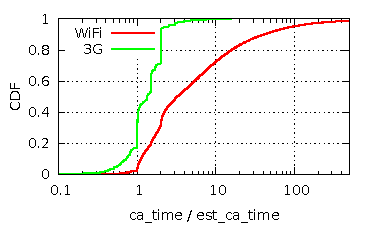
\includegraphics[width=0.8\linewidth]{web_ca_prac_over_est}
\caption{CDF of the extra time introduced by the congestion avoidance stage.}
\label{fig:web_ca_round}
\end{figure}

We first examine how much extra time the congestion avoidance stage introduces for individual flows. Let $\#(ca\_pkts)$ be the number of packets transmitted in this stage for a flow. As a TCP sender, the server sends $cwnd$ packets in one RTT. Thus, if the flow had not experience the congestion avoidance stage, the server would have sent $\#(ca\_pkts)$ packets in a time frame of $T_e = \frac{\#(ca\_pkts)}{cwnd} \times RTT$. Now, we observe the flow actually spent $T_r$ of time for transmitting these packets. Then we compute the ratio of  $T_r$ to $T_e$ and use this ratio to measure the extra time introduced by the this stage. Unfortunately, we are unable to obtain $cwnd$ from the traces and thus alternatively use the number of in-flight packets at the time when entering the stage to approximate this value\cite{rfc56812009tcp}. 
 
Figure \ref{fig:web_ca_round} reports the distribution of this ratio. We observe a surprisingly high ratio for WiFi flows. The median ratio is as high as 3.2 and 20\% of the WiFi flows has a ratio more than 11, meaning a 10 times extra time is introduced for these 20\% of flows. 3G flows on the other hand have a ratio no more than 2 for 95\% of the flows. The difference of 3G and WiFi flows in the packet loss rate (3\% in WiFi versus 0.9\% in 3G) and the difference in the impact of packet loss should contribute most to the huge difference between WiFi and 3G flows observed in Figure  \ref{fig:web_ca_round}. 



\begin{table}[th]
\caption{The finish time (in second, represented as $mean$ ($5th$ percentile, $95th$ percentile)) under different number of lost packets.}
\label{tab:web_loss_finish_time}
\centering
\renewcommand{\arraystretch}{1.0}
\begin{tabular}{c|c|c}
\hline
\#(lost pkts) & WiFi & 3G\\
\hline
0 & 0.18 (0.03, 3.20) & 0.12 (0.01, 0.57) \\
%
1 & 0.48 (0.05, 12.07) & 0.22 (0.04, 0.57) \\
%
2 & 0.54 (0.08, 14.46) & 0.23 (0.04, 0.59) \\
%
$\ge$3 & 2.82 (0.14, 34.89) & 0.27 (0.05, 0.93) \\
\hline
\end{tabular}
\end{table}

We examine the impact of packet loss on finish time in Table \ref{tab:web_loss_finish_time}. Flows are grouped based on how many packets were lost in individual flows. The median of the finish time, along with the $5th$ percentile and $95th$ percentile values of each group are reported. For comparison, we also report the statistics for flows without any packet loss (i.e. these flows finish the data transmission in the slow start stage). For 3G flows, a packet loss increases the flow finish time by about one fold compared to the flows with no packet loss. A higher number of packet loss than 1 does not increase the finish time significantly. Moreover, it seems that packet loss has a higher impact on finish time for WiFi flows than 3G flows. For example, the median finish time increases from 180 ms for flows with no packet loss to 480 ms for flows with 1 lost packets, and grows up to 2.8 second for flows with more than 3 lost packets. 

The huge difference in the impact of packet loss on finish time for WiFi and 3G flows is related to how the packet loss is recovered. A packet loss can be recovered by either fast retransmit, limited retransmit~\cite{allman2001enhancing}, early retransmit~\cite{rfc5827}, or timeout retransmission by the server. \textbf{zhenyu: is there any other recovery method? Do we need to mention the linux version of the server? since the version decides whether tlp or er availability.} {\color{red}{Qinghua: As far as we know, there are the above 4 types of retransmission. Linux version could be mentioned but is not neccesary, as TLP can also be backported into old version Linux kernel. Thus we should point out that TLP is not deployed in the servers.}} Among these possible recovery methods, the most expensive one is the timeout retransmission, which is indeed the factor that explains the difference for WiFi and 3G flows observed in Table \ref{tab:web_loss_finish_time} as our following analysis reveals. 

\subsection{Timeout Retransmission Analysis}

\begin{figure}[th]
\centering
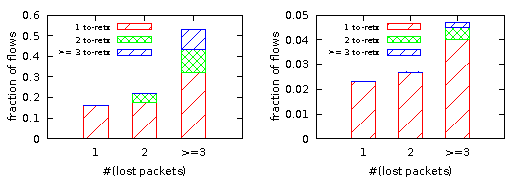
\includegraphics[width=\linewidth]{web_loss_rto_ratio}
\caption{The fraction of flows with timeout retransmission under different number of lost packets.}
\label{fig:web_loss_rto_ratio}
\end{figure}

A retransmission is identified as a timeout retransmission if this retransmission happens at least a time frame of RTO after the transmission of the previous packet. The RTO here is computed as $\text{SRTT} + max(200ms, 4 \text{ RTTVAR})$\cite{rfc62982011computing}, where SRTT is the smoothed value of all RTTs that can be measured accurately from server, and RTTVAR is the variation of RTTs. We examine the fraction of flows that experience timeout retransmission(s) given the number of lost packets in Figure ~\ref{fig:web_loss_rto_ratio}. Note that the two sub-figures have different $y$-axis limitations. We can see that WiFi flows are more likely to suffer from timeout retransmissions than 3G flows. Given the same number of lost packets, the fraction of WiFi flows suffering from timeout retransmissions is about one order of magnitude higher than that of 3G flows. Another notable observation is that 20\% of WiFi flows having more than 3 packets lost experience more than 2 timeout retransmissions, which could lead to a serious performance degradation for these flows. This percentage however is only 1\% for 3G flows. 

An interesting question is then \textit{why the timeout retransmissions are more likely to happen for WiFi flows than 3G flows}. To answer this question, we need to nail down the reasons behind a timeout retransmission. Essentially, there are two scenarios in which a TCP sender has to appeal timeout retransmission for loss recovery. The first scenario is that the retransmitted packet issued for example by fast retransmit to recover the loss is dropped by network. In this case, the sender has to wait for a time frame of RTO to recover the packet loss (referred as \emph{double retransmission}). 

The second scenario is that the sender cannot collect sufficient number of duplicate acknowledgments (\emph{dupacks}) to trigger fast retransmit. The insufficiency of dupacks could be caused by various reasons: (1) the packet loss happens in the last 3 packets of a flow, referred as \emph{tail retransmission}~\cite{flach2013reducing}; (2) the congestion window is small (\eg 1 segment size after timeout retransmission), referred as \emph{small congestion window retransmission}; (3) the lost packet is followed subsequently by other packets with higher sequence numbers and the ACKs of subsequence packets are delayed for a long time (say longer than RTO), referred as \emph{packet delay retransmission}. The last case might be caused by large network latency jitters or by the middleboxes' behavior of blocking the dupacks~\cite{honda2011isit}. 

\begin{algorithm}
	\caption{Process of determining the type of timeout retransmission.}
	\label{alg:rto}
	\begin{algorithmic}[1]
		\Procedure{ParseRTO}{$timeout\ retx$}
			\If {packet has been retransmitted}
				\State \textbf{return} $double\_retransmission$
			\ElsIf {position to tail $\le$ 3}
				\State \textbf{return} $tail\_retransmission$
			\ElsIf {\#(in-flight packets) = 1}
				\State \textbf{return} $small\_cwnd\_retransmission$
			\ElsIf {only 1 in-flight packet is dropped \textbf{and}
				\Statex \indent\indent\indent\indent no dupack is received}
				\State \textbf{return} $packet\_delay\_retransmission$
			\Else
				\State \textbf{return} $others$
			\EndIf
		\EndProcedure
	\end{algorithmic}
\end{algorithm}

We use the method shown in Algorithm~\ref{alg:rto} to determine the type of timeout retransmission. Those that cannot be classified into any of the above type (e.g. when all packets in the windows are dropped) are labeled as others. Table \ref{tab:rto_type} reports the fraction of timeout retransmissions classified into each type.

\begin{table}[th]
\caption{Types of timeout retransmissions.}
\label{tab:rto_type}
\centering
\renewcommand{\arraystretch}{1.0}
\begin{tabular}{c|C{1.1cm}|C{1.1cm}}
	\hline
	{timeout retx type} & WiFi & 3G \\
	\hline
	tail retx & 38.3\% & 69.6\% \\
	%\hline
	double retx & 33.8\% & 13.5\% \\
	%\hline
	packet delay retx & 27.4\% & 16.1\% \\
	%\hline
	small cwnd retrx & 0.3\% & 0.6\% \\
	others & 0.2\% & 0.2\%\\
	\hline
\end{tabular}
\end{table}

Tail retransmission contributes the majority (i.e. 70\%) of timeout retransmissions for 3G flows. Indeed, if the packet loss happens in the tail of a flow, it has to be recovered through timeout retransmission\footnote{The TLP \cite{flach2013reducing} was not enabled in the servers we examined.} Given the small size of web search flows, the tail packet loss can lead to a notable increase of finish time~\cite{flach2013reducing}. However in WiFi flows, only 38\% of the timeout retransmissions are classified as tail retransmissions, because double retransmission and packet delay retransmission become much more important than in the 3G flows. The higher probability of double retransmission in WiFi flows might come from the higher packet loss rate, in which case the retransmitted packet itself is dropped. On the other hand, the higher probability of packet delay retransmission implies a possibility that in WiFi network that we examined, middleboxes might buffer the disordered packets. We leave the examination of middleboxes effect as our future work.

The results in Table \ref{tab:rto_type} explain why timeout retransmissions are more likely to happen in WiFi flows: besides tail retransmissions, the loss of the retransmitted packet and the delayed ACKs also increase the likelihood of timeout retransmission greatly for WiFi flows, but they contribute much less in 3G flows. Our observations also implies that besides the mitigation method (like TLP \cite{flach2013reducing}) for tail retransmission, we also need methods to mitigate the double retransmissions and packet delay retransmissions, especially in WiFi network.

\subsection{Summary of web search analysis}

The key observations on web search flows are summarized below.

\begin{itemize}
	\item RTT plays an important role in the flows experiencing seldom packet loss events. In the flows with lost packets, the time spent on loss recovery dominates the finish time.
	\item More than 50\% of flows spend at least 30\% of their total time on establishing connections.
	\item About 10\% of flows experience packet loss. In WiFi network, 80\% of flows with packet loss drop their packets in the initial congestion window.
	\item Compared with 3G flows, WiFi flows are more sensitive to packet loss. Under the same number of lost packets, WiFi flows experience much longer finish time than 3G flows.
	\item Most of timeout retransmissions in both networks are induced by packet loss at flow tail. However, double retransmission and packet delay retransmission occupy 33.8\% and 27.4\% of timeout retransmissions in WiFi flows.
\end{itemize}
%!TEX root = main.tex

\section{Implication}
\label{sec:implication}


%!TEX root = main.tex

\section{Related Work}
\label{sec:related}

\bibliographystyle{ieeetr}
\bibliography{reference}

\end{document}
